\section{Ext 2/3/4}
\subsection{Introducción}
\begin{frame}{Introducción}
  \begin{itemize}
    \item Surgió como sustituto para el sistema Minix en Linux.
    \item En abril del 92 fue liberado la versión 1 usando ya la API VFS de Linux.
    \item Soluciono gran parte de los problemas que planteaba Minix (Principalmente tamaño máximo y número de caracteres).
    \item En el 93 aparece su versión 2 incorporando ideas de Berkeley Fast File System y pensado para escalabilidad.
  \end{itemize}
\end{frame}

\subsection{Características}
\begin{frame}{Características ext2}
  \begin{itemize}
    \item Permisos POSIX
    \item ACLs
    \item Tamaño máximo: 8TB
    \item Tamaño máximo de fichero: 2TB
    \item Máximo de caracteres de nombre de fichero: 255B
    \item Máximo número de ficheros: NA
  \end{itemize}
\end{frame}

\begin{frame}{Características ext3}
  \begin{itemize}
    \item Journaling
    \item ACLs
    \item Extents (Actualización)
    \item Tamaño máximo: 8TB
    \item Tamaño máximo de fichero: 2TB
    \item Máximo de caracteres de nombre de fichero: 255B
    \item Máximo número de ficheros: NA
  \end{itemize}
\end{frame}

\begin{frame}{Características ext4}
  \begin{itemize}
    \item Journaling
    \item ACLs
    \item Extents
    \item Tamaño máximo: 1EB
    \item Tamaño máximo de fichero: 16TB
    \item Máximo de caracteres de nombre de fichero: 255B
    \item Máximo número de ficheros: 4.000.000.000
  \end{itemize}
\end{frame}

\subsection{Estructura}
\begin{frame}{Estructura}
  \begin{itemize}
    \item Al principio de la partición nos encontramos el sector de arranque.
    \item El resto del espacio (prácticamente todo) se divide en grupos de bloques.
    \item Cada grupo de bloques contiene:
    \begin{itemize}
      \item Si es el primero un superbloque, si no, puede o no contener un backup de el superbloque.
      \item Un descriptor de grupo, que contiene información sobre el grupo de bloques.
      \item Un mapa de bits de bloques, que contiene información sobre los bloques libres.
      \item Un mapa de bits de inodos, que contiene información sobre los inodos libres.
      \item Bloque de datos, que contiene los datos de los ficheros.
    \end{itemize}
  \end{itemize}
\end{frame}

\begin{frame}{Estructura}
  \begin{center}
    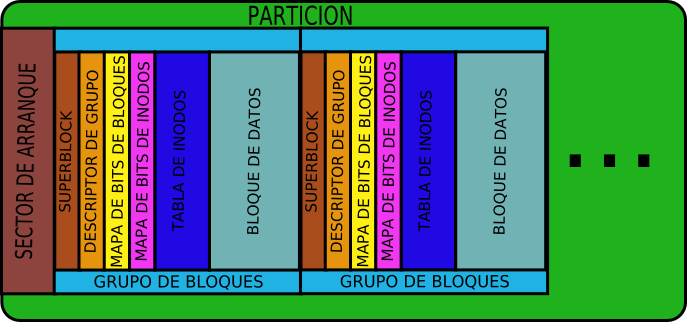
\includegraphics[height=5.5cm]{imgs/ext_struct.png}
  \end{center}
\end{frame}

\begin{frame}{Ficheros}
  \begin{itemize}
    \item La información de los ficheros se almacena en los inodos. Un fichero puede ser un directorio, un fichero regular, un socket, etc...
    \item En el inodo no se almacenan datos, solo punteros a los bloques de datos o extents.
    \item Los punteros a los bloques de datos pueden ser:
    \begin{itemize}
      \item Directos: Apuntan directamente a un bloque de datos
      \item Indirectos: Apuntan a un bloque de punteros directos.
      \item Doblemente indirectos: Apuntan a un bloque de punteros indirectos.
      \item Triplemente indirectos: Apuntan a un bloque de punteros doblemente indirectos.
    \end{itemize}
    \item Los extents se representan dentro de un arbol B+:
    \begin{itemize}
      \item Cualquier nodo intermedio contiene una serie de índices que apuntan a nodos hijos.
      \item Los nodos hoja contienen estructuras extent que apuntan a un conjunto de bloques.
    \end{itemize}
    \item Los datos almacenados en los directorios son el nombre del fichero y el inodo que lo contiene.
  \end{itemize}
\end{frame}

\begin{frame}{Ficheros}
  \begin{center}
    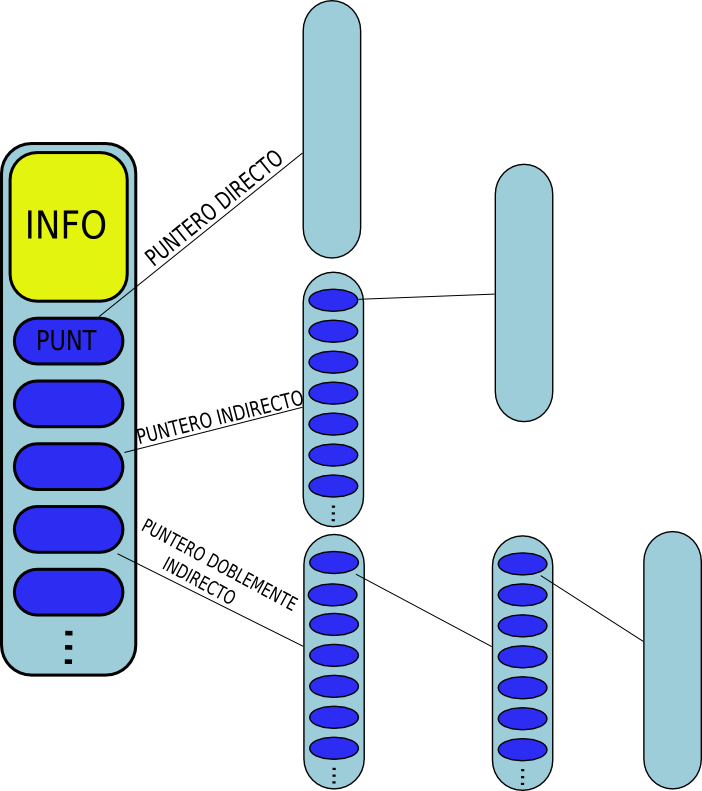
\includegraphics[height=6cm]{imgs/ext_files.png}
  \end{center}
\end{frame}
